\section{Implementation and Evaluation}
\begin{figure}[t]
\centering
\scriptsize
\setlength{\fboxsep}{4pt}

\fbox{%
\begin{minipage}{0.93\linewidth}
\textbf{Model context}\par
\ttfamily
sig User \{\\
\hspace*{1em}follows: set User,\\
\hspace*{1em}sees: set Photo,\\
\hspace*{1em}posts: set Photo,\\
\hspace*{1em}suggested: set User\\
\}\\
sig Influencer extends User \{\}\hspace{1.5em}%
sig Photo \{ date: one Day \}\\
sig Ad extends Photo \{\}\hspace{1.5em}sig Day \{\}
\end{minipage}%
}

\vspace{4pt}

\begin{minipage}[t]{0.47\linewidth}
\raggedright
\textbf{LEFT}\par
\ttfamily
pred left \{\\
\hspace*{1em}all u: User, p: Photo |\\
\hspace*{2em}p in u.sees implies\\
\hspace*{3em}(p not in Ad) implies\\
\hspace*{4em}p in u.follows.posts\\
\hspace*{5em}or p in Ad\\
\}
\end{minipage}
\hfill
\begin{minipage}[t]{0.47\linewidth}
\raggedright
\textbf{RIGHT}\par
\ttfamily
pred right \{\\
\hspace*{1em}all user: User, photo: Photo |\\
\hspace*{2em}photo in user.sees implies\\
\hspace*{3em}photo in user.follows.posts\\
\hspace*{4em}or photo in Ad\\
\}
\end{minipage}

\vspace{4pt}

\begin{minipage}{0.95\linewidth}
Let
\(A(x,y)\equiv y\in x.\mathsf{sees}\),
\(B(x,y)\equiv y\in x.\mathsf{follows}.\mathsf{posts}\), and
\(C(y)\equiv y\in\mathsf{Ad}\).
The typed quotient context is
\(\Gamma_Q=\{q_0:\mathsf{User},q_1:\mathsf{Photo}\}\).

\[
\begin{aligned}
\mathsf{left}
&\stackrel{\mathrm{Imp},\,\alpha_{\Gamma_Q}}{\Longrightarrow}
  \neg A(q_0,q_1)\lor C(q_1)\lor B(q_0,q_1)\lor C(q_1)\\
&\stackrel{\mathrm{ACI}_{\lor}}{\Longrightarrow} Q,
\\[1mm]
\mathsf{right}
&\stackrel{\mathrm{Imp},\,\alpha_{\Gamma_Q}}{\Longrightarrow}
  \neg A(q_0,q_1)\lor B(q_0,q_1)\lor C(q_1)\\
&\stackrel{\mathrm{ACI}_{\lor}}{\Longrightarrow} Q.
\end{aligned}
\]
\end{minipage}

\vspace{2pt}

\fbox{%
\begin{minipage}{0.93\linewidth}
{\centering\textbf{Shared readable quotient}\par}
\ttfamily
all \_q0: User, \_q1: Photo |\\
\hspace*{1em}\_q1 not in \_q0.sees\\
\hspace*{1em}or \_q1 in \_q0.follows.posts\\
\hspace*{1em}or \_q1 in Ad
\end{minipage}%
}

\caption{Schematic certificate-bound saturation of two Alloy
predicates. $\mathrm{Imp}$ denotes certified implication elimination;
$\alpha_{\Gamma_Q}$ admits only type-preserving binder renamings, so
the \texttt{User} and \texttt{Photo} coordinates cannot be exchanged;
and $\mathrm{ACI}_{\lor}$ flattens, reorders, and deduplicates the
visible disjunction children under the declared ACI certificates.
The final Alloy text is a readable projection of the common canonical
observation, rather than an independent authority for equality.}
\label{fig:alloy-certificate-example}
\end{figure}
\label{sec:evaluation}
Figure~\ref{fig:alloy-certificate-example} uses the social-media model
introduced in Section~\ref{sec:background} to compare two predicates for
the same policy. Predicate \texttt{left}
uses a nested implication; after implication elimination, its body
contains two copies of \texttt{p in Ad}. Predicate \texttt{right}
states directly that every seen photo is either posted by a followed
user or is an ad. The implication and ACI steps are admitted only by
their endpoint-indexed certificates, while the $\alpha$-equivalence
step maps \texttt{u}/\texttt{user} to \texttt{\_q0: User} and
\texttt{p}/\texttt{photo} to \texttt{\_q1: Photo} through
type-preserving slot maps. The disjunction port then flattens
association, forgets child order, and removes the duplicate under
idempotence. Both inputs therefore have the readable quotient shown
below. This equality is relative to the declared certified rewrite
theory, not to a complete decision procedure for Alloy.

%\Fix{I am not sure what the following sentence is saying. Is it just saying that we implemented our typed slotted e graphs over the Alloy language? -- Yes} 
We instantiate the representation with Alloy in an environment with a Java backend consisting of an API based on the Kodkod SAT Solver and a parser. The evaluation
asks (1) how much recorded structural variation the implemented observations
consolidate, (2) which transformation families distinguish the evaluated arms,
and (3) at what recorded cost.  Throughout, \emph{canonical} means canonical
only under the implementation's side-conditioned rewrite vocabulary.  The
frozen measurements are manifest-bound observations: the current evidence does
not establish that the Java adapter refines the formal construction, that the
reported equalities are complete for Alloy semantics, or that the corpus has
been replayed by an independently verified checker. 
%\Fix{for the prior sentence, I think this information is also outlined in the background section to a degree. We could reduce redundancy here, although there is enough text in between the two I think it is fine. However, I would say that Java is mentioned without any context. I think it may be good to mention that things were done in Java due to Alloy's source code so that these Java references are not random. If that is mentioend earlier, I missed it. This is probably best mentioned once in the background/scope section.} 
%The values below are
%bound to clean publication run prefix \texttt{db9f89bf} and source-commit
%prefix \texttt{8ad5fead}; Appendix~\ref{app:evaluation-detail} records the
%complete manifest identities and hashes.

\paragraph{Corpus and protocol.}
The classified Alloy4Fun snapshot~\cite{alloy4funDataset2023,alloy4fun,novice} contains 66,080
student--oracle pairs.  Removing 4,482 pairs with identical parsed Abstract Syntax Trees (ASTs) leaves
61,598 pairs: 19,212 labeled \texttt{CORRECT} and 42,386 labeled
overconstrained, underconstrained, or both, in 181 invariant groups and 17
problem variants.  Labels come from the dataset, not from a distance.  The
seven arms are controlled variants of the same Java pipeline, not executions
of external e-graph systems.  Each arm ran once in a fresh process on an AMD
Ryzen~9 9950X3D with 16 workers and an 8~GiB heap cap.  Appendix~\ref{app:evaluation-detail}
records the complete arm definitions, tables, and provenance qualifications.

\paragraph{Observation and equality.}
The pipeline separates an editable repair projection from a deterministic
finite-term equality observation.  On all 61,598 pairs, the mean raw AST has
26.787 nodes and the Certificate-Integrated repair observation has 17.990
units.  The Fast Rewrite Intermediate Representation (IR) normal form averages 18.196 units, and the
Certificate-Integrated materialized canonical-representative tree averages
33.199 nodes; these view-specific sizes are not interchangeable edit budgets.
Within invariant groups, 19,393 recorded truths have 4,496 distinct raw ASTs.
The Certificate-Integrated arm records 2,101 distinct exact observations whose
classes contain 11,382 AST-different equal pairs; Fast Rewrite records 2,136
observations and 10,934 such pairs.  On the paired corpus the
Certificate-Integrated arm assigns zero distance to 4,088 of 19,212
labeled-correct pairs and to none of the 42,386 inherited incorrect pairs.
These are zeroes under the frozen implementation's key, not a refinement proof
or an unbounded semantic soundness result.

\paragraph{Repair distance and coverage.}
For a formula $\varphi$, let $T_\varphi$, $B_\varphi$, and $M_\varphi$ be its
temporal skeleton, binding view, and normalized matrix in the repair
projection.  The reported specification is
\begin{equation}
  d_{\mathrm{repair}}(\varphi,\psi)=
  d_{\mathrm{temp}}(T_\varphi,T_\psi)+
  d_{\mathrm{quant}}(B_\varphi,B_\psi)+
  d_{\mathrm{matrix}}(M_\varphi,M_\psi).
\end{equation}
The coordinates respectively use ordered dynamic programming, exact
type-compatible binder-orbit matching, and carrier-specific sequence,
bag-assignment, set-assignment, or direct-child comparison.
The matrix comparison reuses one binder-owner mapping across every inherited
temporal phase. Proof wrappers,
certificates, rebuild metadata, and support plumbing are absent from the
projection.  The Certificate-Integrated paired mean is 14.022, compared with
13.943 for Fast Rewrite.  Over the 42,386 incorrect predicates, their
respective nearest-truth means are 11.563 and 11.451.

As seen in Figure~\ref{fig:distance-coverage}, at inclusive radii 1, 2, 5, and 10, Certificate-Integrated IR coverage
(blue) is respectively 4.0\%, 10.4\%, 31.0\%, and 59.3\%; raw-AST
coverage (orange) is 8.2\%, 11.7\%, 23.8\%, and 43.0\%.  Each curve uses
its own edit units and independently
selects the nearest AST-distinct recorded truth in the same invariant group;
the vertical difference is therefore not an equal-budget improvement.
Unlike mutation-based specification repair~\cite{mutrepair}, this study does not generate or execute the repair candidates. 
%\Fix{The prior sentence was not clear to me but I think this captures the intent.}

\begin{figure}[t]
\centering
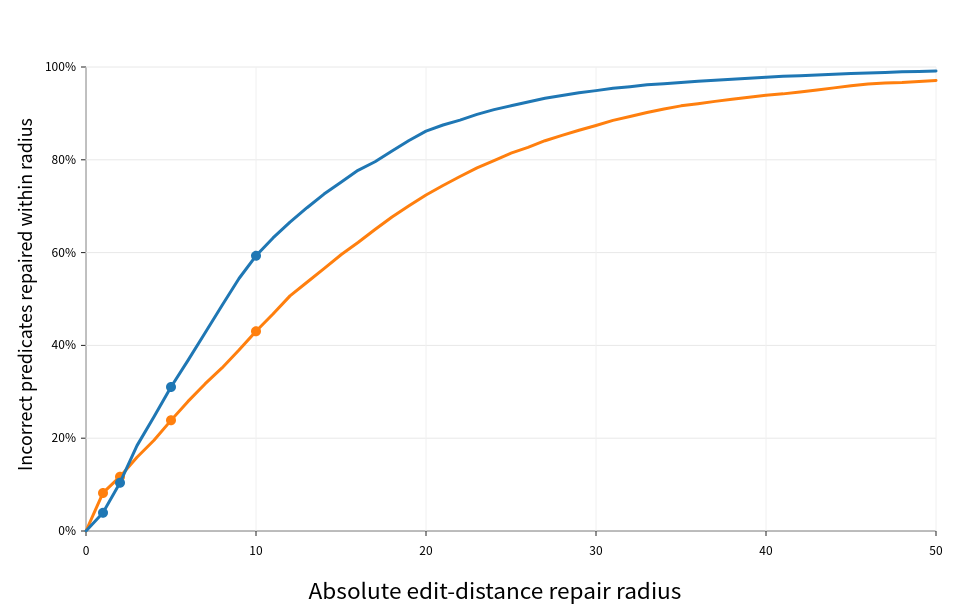
\includegraphics[width={0.78\linewidth}]{figures/raw_edit_repair_coverage_relabel.png}
\caption{Cumulative nearest-reference coverage for the $n=42{,}386$
non-\texttt{CORRECT} predicates.  At inclusive radius $r$, blue is the
Certificate-Integrated IR observation distance and orange is raw-AST tree-edit
distance to the nearest AST-distinct oracle or \texttt{CORRECT} student predicate in
the same invariant group.  The horizontal axis is capped at 50 while all
42,386 predicates remain in the denominator. 
% Trimmed for space, this is outlined in the text already
``Repaired'' in the axis label
denotes only falling within this nearest-reference radius.
%: no candidate is
%generated or executed, and the curves do not measure operational repair
%success.
}
\label{fig:distance-coverage}
\end{figure}


\paragraph{Ablation, capability, and cost.}
Table~\ref{tab:eval-headline} displays the comparisons needed to interpret the
main claims; the full seven-arm ablation and all eleven transformation rows
appear in Appendix~\ref{app:evaluation-detail}.  De Bruijn storage raises the
raw arm's labeled-correct zeroes from 820 to 2,160, whereas the slot-shaped arm
records 2,159.  On the targeted 5,500-pair suite, however, the slot-shaped,
Fast Rewrite, and Certificate-Integrated arms recognize every pair.
Binder-block permutation is the discriminating family: the De Bruijn arm
recognizes 22/500 and each slot-aware arm 500/500.  These are in-vocabulary
recognition results, not completeness or prevalence estimates.

\begin{table}[t]
\centering
\caption{Headline manifest-bound results.  Natural-corpus zeroes and wall time use
61,598 AST-different pairs; targeted recognition uses 5,500 generated,
side-conditioned pairs.  All distances and times are arm-specific.}
\label{tab:eval-headline}
\scriptsize
\setlength{\tabcolsep}{3.3pt}
\begin{tabular}{@{}lrrrr@{}}
\toprule
Arm & Correct $d=0$ & Incorrect $d=0$ & Wall (s) & Targeted\\
\midrule
Raw + De Bruijn & 2,160 & 0 & 19.380 & 3,628/5,500\\
Slot-shaped core & 2,159 & 0 & 19.670 & 5,500/5,500\\
Fast Rewrite IR & 4,074 & 0 & 23.990 & 5,500/5,500\\
Certificate-Integrated & 4,088 & 0 & 2,684.110 & 5,500/5,500\\
\bottomrule
\end{tabular}
\end{table}

The Certificate-Integrated arm behaves as an auditor rather than as a
like-for-like canonicalizer.  For each predicate,  the arm  runs Fast Rewrite IR
and then reconstructs an in-process certificate-checked typed slotted graph.
Each certified mutation validates types and slot contexts,
source-occurrence and binder metadata, and law authority.  Insertions and
rebuild steps invoke whole-state invariant checking, including certificate and
provenance ledgers; congruence merges can re-dirty earlier parent records,
producing a superlinear worst-case work pattern.

The path also enumerates complete bounded finite unfoldings and materializes
proof-heavy construction artifacts.  Several certificate families are
occurrence-bound, while memoization is local to one adaptation, so these
objects cannot be reused wholesale across predicates.  The measured path did
not retain an independent replay trace.  With 16 workers, the certificate-integrated pass  
%\Fix{replace it with the object name directly}
reaches 7,137.811~MiB peak used heap and 8,943.988~MiB maximum Resident Set Size (RSS).  %No GC-pause or object-allocation profile was collected, so the measurements do not attribute a quantified share of the slowdown to garbage collection.

Against Fast Rewrite on the same snapshot, this arm took 111.885 times as much
process wall time and used 593.026 times as much engine CPU; on the targeted
suite the process-wall ratio was 86.920. The Certificate-Integrated arm shows the 
%\Fix{Can we replace its with the object in reference?} 
average pair-level ablation
representation-unit count slightly smaller, 29.541 versus 30.001.  The observed gap is therefore
consistent with this audit-heavy implementation---global validation, exact
renaming and certificate work, rebuilds, and finite unfolding---rather than
representation growth or a different repair objective.  It is not evidence
of an inherent cost of typed e-graphs or the repair metric, nor an
external-system ranking.

\paragraph{Independent checks and limits.}
A separate verifier reconstructs typed judgments, graph checkpoints,
canonical orbits, and finite unfoldings from closed bundles.  Separately, Lean
checks one fixed nontrivial abstract trace comprising AC reassociation, a
bijective two-slot binder remapping, union insertion, rebuild, and congruence
restoration after operand reordering: its indexed construction enforces exact
adjacency, and replay under its supplied finite-set interpreter proves
endpoint-denotation equality.  This witness establishes neither Java
producer--verifier correspondence nor coverage of other trace shapes.  The
corpus used in-process
checks rather than complete exported-and-replayed traces.  

A manifest-bound
bounded Alloy analysis covered the union of 4,088 current correct-pair
zero-distance claim identities from the Fast Rewrite and
Certificate-Integrated arms. Its supported analyses found no counterexample
or solver error and rejected four deliberately invalid probes. A separate
validation refresh checked one generated example from each of 29
family/subtype combinations, with no counterexample, solver error, or
inconclusive result. Eight checks used bounded temporal solving at object
scope 4 and trace bounds 1--10. This refresh fixes temporal-mode detection
through predicate calls and supersedes the six previously inconclusive
temporal checks; it does not replace the full-corpus measurements.
Newer repository packages also check bounded Java-to-Lean constructor and
certificate-record replays, separately from these corpus observations. 

Overall, full Java--Lean refinement,
full-trace replay, semantic completeness, industrial generalization, and
causal attribution remain future work. 


%Consequently, 
%the evaluation supports bounded structural-consolidation and
%transformation-recognition observations only; 
%full Java--Lean refinement,
%full-trace replay, semantic completeness, industrial generalization, and
%causal attribution remain open. 
